% mm comments and significant changes noted like this.


%rnaastex.cls is the classfile used for Research Notes. It is derived
%% from aastex61.cls with a few tweaks to allow for the unique format required.
%% (10/15/17)
%% (01/08/18)
\documentclass[twocolumn]{aastex62}
%\pdfoutput=1 %for arXiv submission
\usepackage{amsmath,amstext}
\usepackage[T1]{fontenc}
\usepackage{apjfonts}
\usepackage[figure,figure*]{hypcap}
%\usepackage{deluxetable}

\renewcommand*{\sectionautorefname}{Section} %for \autoref
\renewcommand*{\subsectionautorefname}{Section} %for \autoref

% citation for method paper
\newcommand{\methodpaper}{Paper I}

% line colors
\newcommand{\fiducialstyle}{black, solid}
\newcommand{\snionstyle}{orange, solid}
\newcommand{\snpelwstyle}{orange, dashed}
\newcommand{\snonly}{orange, dotted}

\newcommand{\shortradstyle}{blue, solid}
\newcommand{\RPzerostyle}{green, solid} 

\newcommand{\radstyle}{red, solid}
\newcommand{\ionstyle}{red, dotted}
\newcommand{\pelwstyle}{red, dashed}

\newcommand{\sfrunits}{M$_{\odot}$~yr$^{-1}$}

\newcommand{\HI}{HI}

%comment commands:
\newcommand{\aje}[1]{\textcolor{blue}{\textbf{(AJE: #1)}}}


%% Define new commands here
\newcommand\latex{La\TeX}

%% Tells LaTeX to search for image files in the 
%% current directory as well as in the figures/ folder.
%\graphicspath{{./}{figures}}

\begin{document}

\title{The Role of Stellar Feedback in the Chemical Evolution in a Low Mass Dwarf Galaxy}

%% Note that the corresponding author command and emails has to come
%% before everything else. Also place all the emails in the \email
%% command instead of using multiple \email calls.
\correspondingauthor{Andrew Emerick}
\email{aemerick@carnegiescience.edu}

%\author{}
%\altaffiliation{}
%\affiliation{}
%% The \author command can take an optional ORCID.
\author[0000-0003-2807-328X]{Andrew Emerick}
\altaffiliation{Carnegie Fellow in Theoretical Astrophysics}
\affiliation{Carnegie Observatories, Pasadena, CA, 91101, USA}
\affiliation{TAPIR, California Institute of Technology, Pasadena, CA, 91125, USA}
\author[0000-0003-2630-9228]{Greg L. Bryan}
\affiliation{Department of Astronomy, Columbia University, New York, NY, 10027, USA}
\affiliation{Center for Computational Astrophysics, Flatiron Institute, 162 5th Ave, New York, NY, 10010, USA}
\author[0000-0003-0064-4060]{Mordecai-Mark Mac Low}
\affiliation{Department of Astrophysics, American Museum of Natural History, New York, NY, 10024, USA}
\affiliation{Department of Astronomy, Columbia University, New York, NY, 10027, USA}
\affiliation{Center for Computational Astrophysics, Flatiron Institute, 162 5th Ave, New York, NY, 10010, USA}


\keywords{Galaxy chemical evolution -- Dwarf galaxies -- Chemical enrichment -- Hydrodynamics}


\begin{abstract}
\textbf{NOTE: I haven't settled on line styles for everything yet, but I was spending far too long figuring out whats best and not enough time writing...}
\end{abstract}

\section{Introduction}
feedback is important for galaxy evolution, but how does it affect low mass dwarfs (ref Hu+, Forbes+, FIRE, changa stuff), and (NEW) how does it affect chemical evolution properties (metal outflows and abundance spreads).

This work builds upon the simulations presented in \citet{Emerick2019} (hereafter, Paper~I)...

\section{Methods} 
\label{sec:methods}
We refer the reader to Paper I for a detailed description of our numerical methods, initial conditions, and feedback and chemical evolution model. We briefly summarize the key components of these methods most relevant to this work below. 

We follows the evolution of an idealized, isolated, low-mass dwarf galaxy with an initial gas mass of $M_{\rm gas} = 1.80 \times 10^6$~M$_{\odot}$ initialized as an exponential disk with radial and vertical scale heights of 250~pc and 100~pc respectively. This galaxy is embedded in a static, \cite{Burkert1995} dark matter potential with virial mass and radius $M_{\rm vir} = 2.48\times 10^{9}~M_{\odot}$ and $R_{\rm vir}~=~27.4$~kpc. This is evolved using the adaptive mesh refinement hydrodynamics code \textsc{Enzo} \citep{Enzo2014}, with a minimum/maximum spatial resolution of 921.6~pc / 1.8~pc in the simulations presented in Paper I. Due to computational constraints, we were unable to perform this study at full resolution, and instead adopt 3.6~pc as the maximum resolution. We refer the reader to the resolution studies comparing maximum resolutions of 1.8~pc, 3.6~pc, and 7.2~pc performed in Paper I and \cite{Emerick2018b}. % I may need to say more here about what exactly the resolution studies show. Mostly 1.8 / 3.6 is OK but definitely large difference moving to 7.2 pc. 
The grid is refined to maintain a mass resolution of 50~M$_{\odot}$ per cell, and to ensure that the Jeans length is resolved by at least eight cells. In addition, a three-zone radius region around any star particle that has active feedback (stellar winds or SNe) is refined to the maximum grid resolution. We use the chemistry and cooling package \textsc{Grackle} \citep{GrackleMethod} to solve a nine species non-equillibrium chemistry model that includes gas-phase and dust H$_2$ formation, a uniform UV background, and localized self-shielding. This galaxy has an initial total metal mass fraction of $5.4 \times 10^{-4}$ (or $0.03 Z_{\odot}$ taking $Z_{\odot}$ = 0.018 from \cite{Asplund2009}). We follow the evolution of 15 individual metal species, C, N, O, Na, Mg, Si, S, Ca, Mn, Fe, Ni, As, Sr, Y, and Ba, whose initial mass fractions are initialized to near-zero (10$^{-20}$). Only the total metallicity affects the physics in our simulation, not the individual metal abundances. 

\subsection{Star Formation and Stellar Feedback}
\label{sec:sf feedback}

Our simulation stochastically forms star particles in dense gas ($n > 50$~cm$^{-3}$ in the 3.6~pc resolution runs presented here) by randomly sampling a \cite{Salpeter1955} IMF and depositing individual star particles from 1~M$_{\odot}$ to 100~M$_{\odot}$. For stars above 8~M$_{\odot}$, we follow their H~{\sc i} and He~{\sc i} ionizing radiation using the adaptive ray-tracing radiative transfer method of \cite{WiseAbel2011}, and trace their radiation in the Lyman-Werner and FUV bands using an optically thin approximation. These stars eject mass and energy over their lifetimes through stellar winds, and we include mass and thermal energy injection of both core collapse and Type Ia SNe. Stars below 8~M$_{\odot}$ have no feedback during their lifetime, except mass and energy deposition of their AGB winds at the end of their life. For stellar winds and SNe, mass, energy, and metals are injected to the grid by mapping a three-cell spherical region ($r=3 \times dx = 7.2~$pc) to the grid using a cloud-in-cell interpolation scheme. To reduce the significant computational expense of following a continuous source of hot ($T > 10^6$~K), fast ($v \sim 10^{3}$~km~s$^{-1}$) moving gas, we greatly reduce all stellar wind velocities to 10~km~s$^{-1}$. Given this reduction, we cannot make any strong statements as to the role of stellar wind feedback in the evolution of low mass dwarf galaxies. 

Both HI and HeI ionizing radiation is followed using the adaptive ray-tracing radiative transfer method of \cite{WiseAbel2011} and coupled to the non-equillibrium chemistry and cooling / heating routines in \textsc{GRACKLE}. Stars in our simulation use the \textsc{OSTAR2002} \citep{Lanz2003} grid of O-type stellar models to compute the HI, HeI, FUV, and LW band fluxes as a function of stellar surface gravity and surface temperature. These latter two quantities, in addition to stellar radius, are taken as a function of mass and metallicity from the \textsc{Parsec} \citep{Bressan2012,Tang2014} grid of stellar models. For stars with stellar properties off of the \textsc{OSTAR2002} grid, we adopt the associated black body flux given the stellar surface temperature. The resulting black body fluxes were adjusted to produce a continuous curve of flux as a function of stellar mass, separately in each band. Rather than adopting fixed HI and HeI photon energies for each star, we adopt the average photon energy weighted by the associated black body curve in each band, leading to HI and HeI ionzing photon energies that span the range 13.6-22.5~eV and 25.0-32.5~eV respectively, depending on stellar surface temperature. We refer the reader to Appendix~B of Paper I which contains plots of each of these quantities. In our fiducial simulations, we include the effects of radiation pressure on \HI but ignore the absorption of ionizing radiation by dust and re-radiation in the infrared.

We assume FUV and LW band radiation are both optically thin, with local (cell-by-cell) attenuation. LW radiation causes $H_2$ dissociation, while FUV radiation leads to PE heating of dust grains. We follow the PE heating models from \cite{Wolfire2003} and assuming the dust-to-gas scaling with metallicity in \cite{Remy-Ruyer2014} which shows a significant decline in the dust content at low-metallicities ($Z < 0.1$~Z$_{\odot}$). Our photoelectric heating rate is given as
\begin{equation}
    \Gamma_{\rm PE} = (1.3 \times 10^{-24} \rm{erg s^{-1} cm^{-3}}) \epsilon n_{\rm H} G_{\rm eff} D
\end{equation}
where $\epsilon$ is an efficiency factor that in detail depends upon $G_o$, temperature, and the electron number density, but which we adopt to scale weakly with $n_{\rm H}$ (see Paper I), $D$ is the dust-to-gas ratio, and
\begin{equation}
    G_{\rm eff} = G_o \rm{exp}(-1.33\times 10^{-21} D N_{\rm H})
\end{equation}
is the locally-attenuated FUV flux. $G_o$ is the FUV flux normalized to the solar neighborhood \citep{Habing1968} and $D$ is normalized to the solar value, 6.617 $\times 10^{-3}$. This model is similar to that used in both \cite{Forbes2016} and \cite{Hu2017}, with the exception of the treatment of $\epsilon$ and $D$. However, we note that both of their galaxies were at or above the $Z > 0.1$~Z$_{\odot}$ threshold and therefore have a significantly higher (but still low) dust content. We do not account for $H^-$ photodetachment due to the ISRF, which plays an important role in producing $H_2$ in our low-metallicity, low-dust content galaxy. However, we find that this effect is likely subdominant as long as either ionization or LW radiation are followed (see Appendix E of Paper I).

\section{Simulations}
\label{sec:runs}

We present the 13 different simulations run varying feedback effects in Table~\ref{table:runs}. Each simulation turns on / off various feedback processes as shown in the table. In each case, both supernovae and stellar winds are included as a pair in each simulation, though again we note that we do not fully capture the effects of stellar winds in our simulations. All runs contain the same total metal enrichment from SN, massive star stellar winds, and AGB winds. In runs without SN and stellar winds, the mass and metal ejecta from these channels are instead injected at low velocity (10 km~s$^{-1}$) with a thermal energy equal to the stellar surface temperature. All runs with ionizing radiation include radiation pressure on \HI. We test the role of radiation pressure by varying its strength with a constant factor in runs RPx2 and RPx5, and turning it off in run RPx0. The shortrad simulation is the same as the fiducial simulation, but photons are deleted once they have travelled more than 20~pc from their source. This is an attempt to approximate localized prescriptions for ionizing radiation feedback which only deposit energy / ionize gas in a localized region around a star particle. We examine the effects of stellar ionizing radiation in our high-resolution (1.8~pc) simulations in \cite{Emerick2018a}, comparing our fiducial run with a shortrad simulation and a simulation without ionizing radiation (i.e. SN+PE+LW), each at 1.8~pc resolution.

% but differs only in the assumed efficiency parameter ($\epsilon$). \cite{Forbes2016} adopts a constant $\epsilon$ (\aje{I'm not sure the exact value}) while \cite{Hu2017} uses the full temperature and electron number density ($n_e$) dependent form from \cite{Wolfire2003}. However, we do not follow the necessary carbon chemistry needed to accurately follow $n_e$ in dense, neutral regions. Instead, we adopt a weak power-law fit in $n_H$ 

\begin{deluxetable*}{c|c|c|c|c|c|c}
\label{table:runs}
\tablecaption{A list of the feedback physics included in each of our runs. In every case, metal enrichment from SNe and stellar winds are kept fixed. Runs with SNe and stellar winds turned off simply replace the proper energy injection with return equal to the stellar surface temperature. The Shortrad simulation does include full radiative transfer, but deletes photons once they have travelled XX~pc from their source. The final column lists the final run time of each simulation. \aje{Starred need to be updated, XX's are still running}}
\tablehead{
\colhead{Run Name} & \colhead{SN} & \colhead{Stellar Winds} & \colhead{Ionizing Radiation} & \colhead{PE Heating + LW Radiation} & \colhead{Radiation Pressure Factor} & \colhead{End Time (Myr)}
}
\startdata
 Fiducial & Yes & Yes & Yes & Yes & 1  & 649* \\
 SN+Ion   & Yes & Yes & Yes & No  & 1  & 767 \\
 SN+PE+LW & Yes & Yes & No  & Yes & 1  & 421* \\
 SN-only  & Yes & Yes & No  & No  & -  & 121 \\
 No PE & Yes & Yes & Yes & LW only & - & XXXX \\
 No LW & Yes & Yes & Yes & PE only & - & XXXX \\ 
 RPx0     & Yes & Yes & Yes & Yes & 0  & 739 \\
 RPx2     & Yes & Yes & Yes & Yes & 2  & 757 \\
 RPx5     & Yes & Yes & Yes & Yes & 5  & 471 \\
 Shortrad & Yes & Yes & Yes* & Yes & 1  & 271** \\
 Radiation Only & No & No & Yes & Yes & 1 & 857 \\ 
 Ionization Only & No & No & Yes & No & 1 & 920 \\ 
 PE+LW Only & No & No & No & Yes & - & 521 
\enddata
 
\end{deluxetable*}

\section{Results}

\subsection{Star Formation Regulation}
\label{sec:sfr}

In Figure~\ref{fig:SFR} we compare the star formation rate as a function of time for each of our runs. As discussed in \methodpaper, the SFR evolution for the higher resolution fiducial simulation exhibits an initial burst up to 10$^{-3}$~M$_{\odot}$~yr$^{-1}$ followed by a lower-average, bursty SFR ($<$SFR$> = 1.19\times 10^{-4}$~M$_{\odot}$~yr$^{-1}$) with periods of up to 50-100~Myr with no star formation. This behavior is found also in the lower resolution fiducial simulation shown here (\fiducialstyle).\footnote{Our star formation algorithm has a minimum threshold gas mass to convert into stars in a single time-step, 100~$M_{\odot}$. SFR here is plotted in 10~Myr bins, yielding an effective SFR floor of $10^{-6}$ \sfrunits in Figure~\ref{fig:SFR}.} The most immediately visible difference between each of the runs is the magnitude of the initial burst of star formation in the first $\sim$100~Myr. This is the largest for SN-only (\snstyle), which contains no ionizing radiation, and becomes smaller when turning on radiation. Inclusion of PE heating and LW radiation in SN+PW+LW (\snpelwstyle) brings this down by a factor of $\sim$3.5, while ionizing radiation in SN+Ion (\snionstyle) has a larger effect, recovering nearly the same burst as the fiducial simulation. Interestingly, the simulations without SN (right panel) all show about the same peak SFR as the fiducial simulation. This is a clear indication that pre-SN feedback through radiation is important for star formation regulation. During this initial phase, these runs show that, while together PE heating and LW radiation do have an effect on the SFR in the absence of ionizing radiation, ionizing radiation dominates when all three effects are included.

\begin{figure*}
  \centering
  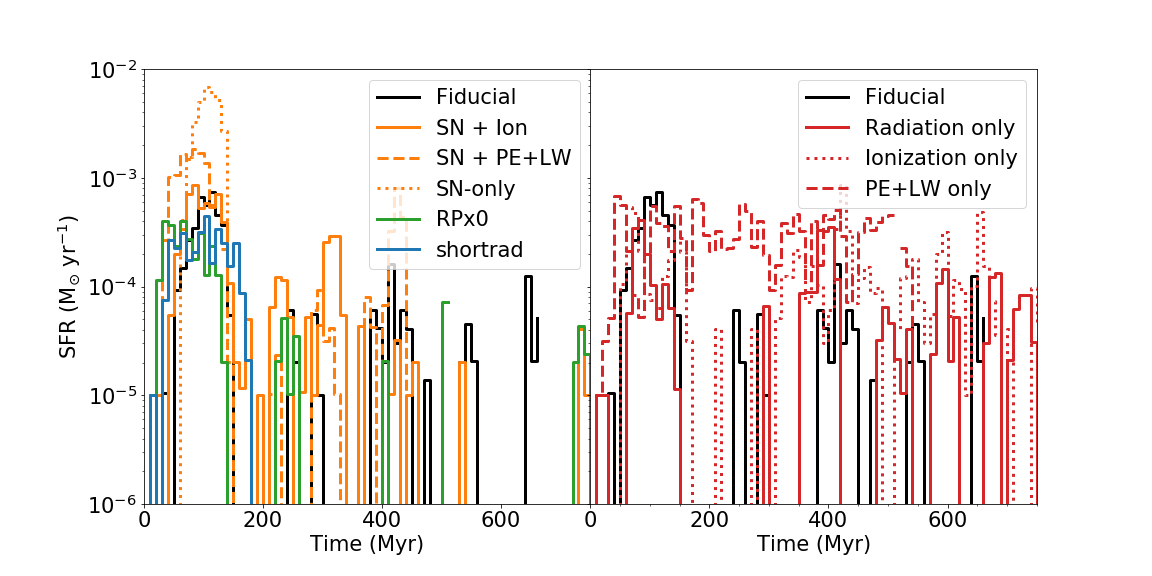
\includegraphics[width=0.98\linewidth]{figures/physics_comparison_sfr_2}
  \caption{The SFR in each of our runs, comparing those with SN feedback (left) to those without SN (right). The fiducial simulation, which includes all physics, is plotted in both panels (\fiducialstyle) for comparison.}
  \label{fig:SFR}
\end{figure*}

After the first 100~Myr, the differences between runs by the inclusion of SN feedback becomes obvious. Each of the SN-included runs (left panel) show various degrees of bursty star formation for the remainder of the simulation time, with lower average star formation rate than the ionization runs. The run with only PE heating and LW radiation, PE+LW (\pelwstyle), shows the most steady SFR, indicating that this feedback channel alone is capable of producing a self-regulating SFR in this galaxy, but not the bursty star formation that is seen with the inclusion of any other feedback channel. Ionization alone (\ionstyle) and the combined radiation run (\radstyle) both show burst star formation like the SN runs, but still have a higher average SFR and more consistent SF through the end of the simulation. The SN runs have progressively lower SFR and longer quiescent periods as each simulation proceeds.

(\aje{Maybe show summary table of comparison values? average SFR, average retention fractions, average outflow, etc.?... maybe do this in discussion?})

\subsection{Galaxy Morphology}

\begin{figure*}
  \centering
  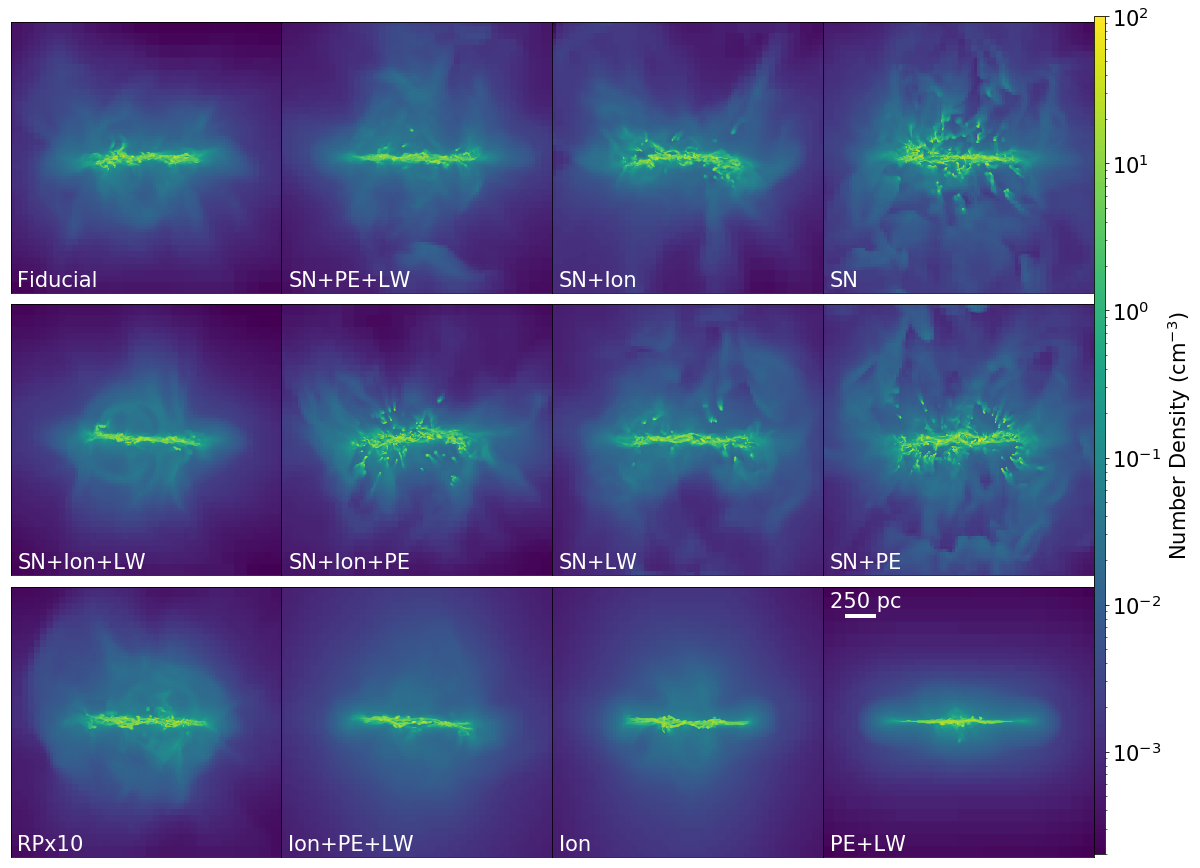
\includegraphics[width=0.95\linewidth]{figures/proj_plot_n_x_125.png}
  \caption{Edge-on projections of gas number density for each of our runs at time $t=125$~Myr.}
  \label{fig:panel_plot_1}
\end{figure*}

\begin{figure*}
  \centering
  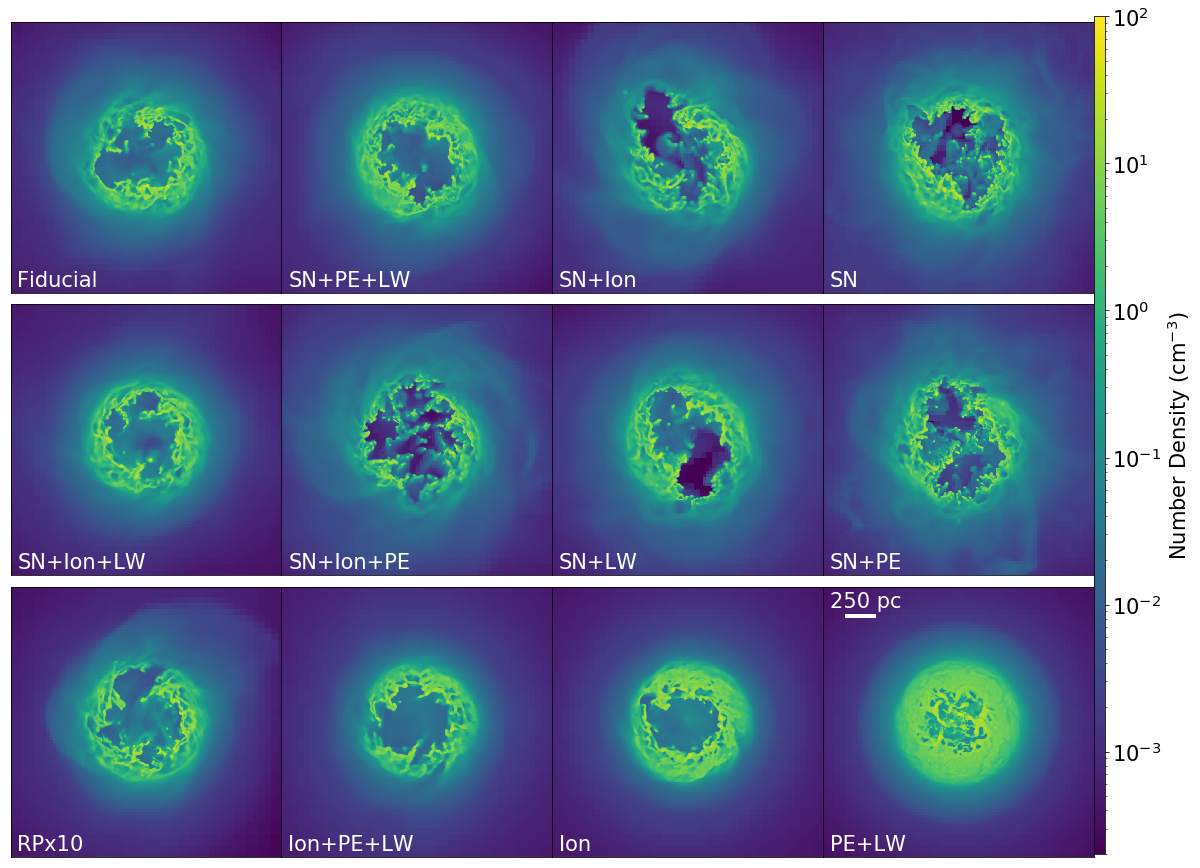
\includegraphics[width=0.95\linewidth]{figures/proj_plot_n_z_125.png}
  \caption{The same panels as Figure~\ref{fig:panel_plot_1}, but face-on.}
  \label{fig:panel_plot_2}
\end{figure*}

We show a comparison of gas morphology of our low-mass dwarf galaxy in edge-on and face-on density-weighted projects of gas number density in Figure~\ref{fig:panel_plot_1} and Figure~\ref{fig:panel_plot_2} respectively at 125~Myr for each simulation. In every simulation with SNe (top two rows), the gas disk is puffier with a larger scale height, and with significant diffuse, outflowing gas above and below the disk. This is not true for the runs with only radiation (bottom row), which exhibit thin disks with no significant outflowing gas, though ionizing radiation is capable of heating the disk somewhat. Interestingly, some of the runs show many small ($\sim$10~pc), dense clumps of gas above / below the disk (most significantly, SN+Ion and SN-only). Based upon visual analysis the evolution of these panels, these clumps are dense clumps of gas from the ISM that are entrained in the outflows. These clumps are still bound to the galaxy, and are ablated by the more rapidly moving diffuse gas outflows, giving rise to trailing tails behind the clumps. In some cases these clumps are fully ablated and destroyed, while in others they persist, remain bound to the galaxy, and fall back in on a larger orbit with much larger azimuthal motions. These clumps do appear at some point in all simulations with either SNe or ionizing radiation, but to a much smaller extent than the obvious cases shown here. Our higher resolution fiducial simulation presented in Paper~I did show some of these features, but again not to the extreme shown here. SN+Ion and SN-only have the most disturbed, disk mythologies. 

In the face-on panels, each galaxy with SNe or ionizing radiation shows a low-density, carved-out circular region at the center, surrounded by a ring of dense gas. The lack of gas in the center of each galaxy is a particular consequence of the large initial burst of star formation present in every case. However, the stellar feedback from SNe and ionization radiation are (alone and together) effective at heating up and driving out cold ISM in the center of galaxy as stars form, which leads to a reduction of the central gas content even outside of this burst phase. Only the Pe+LW run is incapable of removing gas from the center, maintaining a more more uniform and more massive gas disk with localized patches of diffuse gas around newly formed stars. Most of the clumps seen within the diffuse central region in each simulation are there as projection effects, and lying outside the mid-plane of the galaxy. 



\subsection{Global Galaxy Properties}
\label{sec:galaxy properties}

In Figure~\ref{fig:properties} we compare the time evolution of the total \HI mass, stellar mass, H$_2$ mass fraction, and average ISM metallicity for each of our runs. The \HI mass in the fiducial simulation declines with time as stars form, radiation ionizes the ISM, and SN feedback drives significant mass loss. Interestingly the H$_2$ fraction increases significantly during this time, but, as shown in Paper~I, this is mostly due to the preferential retention of the cold, dense gas where the H$_2$ resides, rather than the generation of a significant amount of mass of molecular hydrogen. In the bottom right panel we show the evolution of only those metals self-consistently produced by stars formed in the simulation; the initial metal fraction for these species is 10$^{-20}$. In the fiducial run, the mean ISM metallicity remains well below what could be expected for a closed-box model (black, dashed). As discussed in Section~\ref{sec:outflows} this is due to the significant outflows generated by feedback in this galaxy. 

\begin{figure*}
  \centering
  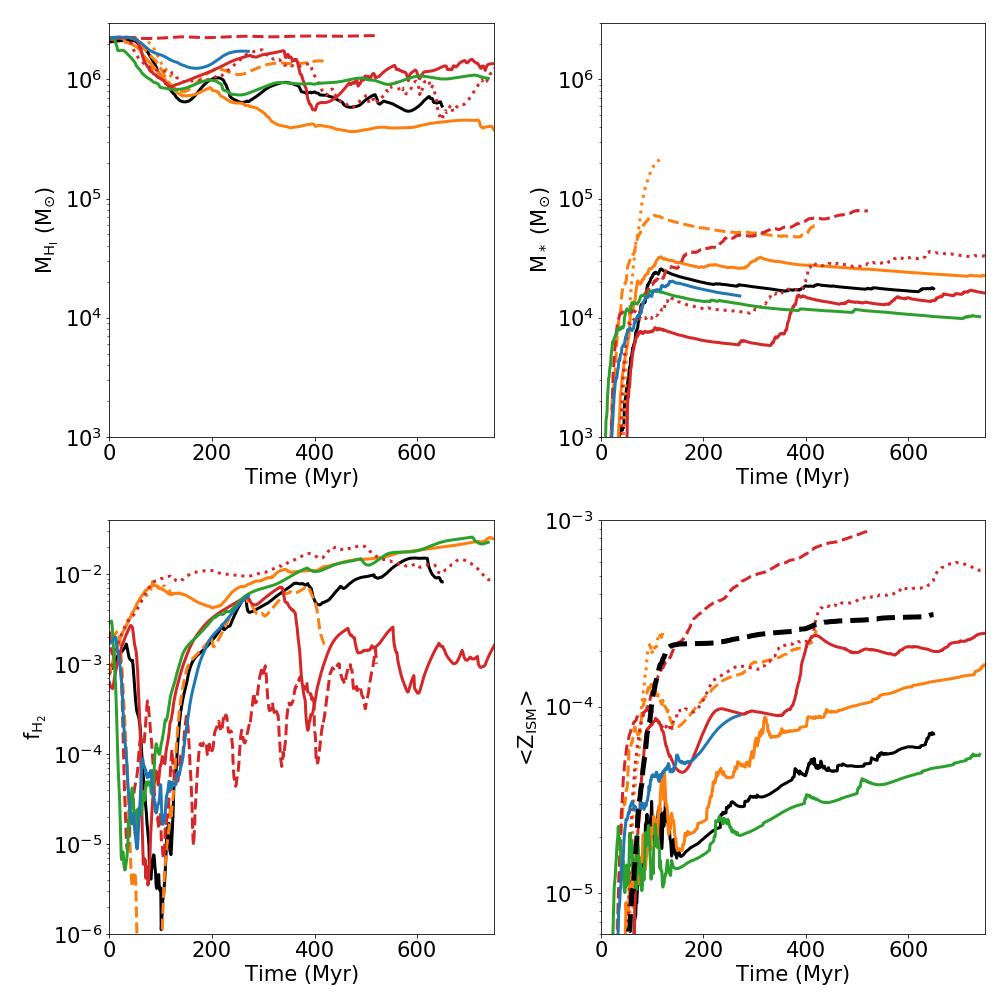
\includegraphics[width=0.98\linewidth]{figures/physics_comparison_masses}
  \caption{The evolution of four global galaxy properties for each of our simulations. Clockwise from top left: \HI mass, stellar mass, H$_2$ fraction, and mean ISM metallicity. $M_{\rm \HI}$ and $M_{*}$ have the same vertical axis limits for comparison of the stellar mass fraction between runs. The $<Z_{\rm ISM}>$ shown here only includes metals self-consistently produced by stars in this simulation (see text).
  \aje{Include legend again?}}
  \label{fig:properties}
\end{figure*}

SN+Ion produces the lowest \HI mass of all of the runs. Compared to the fiducial simulation, this is likely due to the increase in stellar mass and increase in number of ionizing photons (\aje{though maybe also outflows...check later}). Each of the other simulations have a higher \HI mass, in spite of the fact that most have higher total stellar masses. The common theme among these runs is the lack of ionizing radiation, which, along with outflows, is clearly important for regulating the neutral gas fraction of this galaxy. The importance of outflows in regulating the gas content can be seen by comparing the radiation only (\radstyle) run to the fiducial, which shows a similar total stellar mass but greater \HI content, and the ionization only run (\ionstyle) which has a stellar mass higher than both the fiducial and SN+Ion runs but a comparable \HI mass to the fiducial run. At the extreme, PE+LW radiation alone clearly is incapable of ionizing or removing any \HI from this galaxy, in spite of its comparatively high stellar mass. Interestingly, the total stellar mass for the SN+PE+LW run is similar to that with PE+LW alone -- further indicating that PE+LW are not significant sources of pre-SN feedback compared to ionizing radiation -- but has a lower \HI mass, likely due to SN-driven outflows. Wewill discuss outflows in more detail in Section~\ref{sec:outflows}.

\aje{It may be worth exploring in more detail why the radiation run and ionization only runs have lower stellar masses for first few Myr than the fiducial.}

With the exception of the radiation (\radstyle) and PW+LW (\pelwstyle) runs, the molecular hydrogen fraction is quite similar throughout the galaxy's evolution. What is most clear from this plot is that stellar LW radiation is indeed important to consider if attempting to model the molecular gas content. The two runs without LW radiation (SN+Ion and ionization-only) show fewer fluctuations in the molecular gas content than the other runs, most obvious during the initial 100~Myr burst where the $H_2$ fractions drop dramatically for those runs with LW radiation. \aje{not sure if need more here? also not sure if it would be better to plot H2 mass to remove the evolution of the denominator from the interpretation?}

Understandably, the differences in stellar mass evolution and gas content in these runs leads to a significant variation in the mean ISM metal fraction. The fiducial run 

\subsection{Multi-Phase Gas}
%\aje{Its a bit hard to be very precise about this comparison since it's not easy to distinguish feedback effects directly from there just being less / more SF and SNe due to changes in effectiveness of feedback (best example is the RPx0 comparison... I'd expect very little differences, but there are some and its likely not due to lack of RP, but more likely to due sligly different SFR over this time)....might be worth mentioning this as a caution?:}
The properties of the multi-phase ISM for our galaxy simulations is feedback-driven as shown in the temperature-density phase diagrams Figure~\ref{fig:phase_diagram}, and the 1D temperature and density PDFs in Figure~\ref{fig:1D_phase}. Both figures show only gas contained within the disk of each galaxy, and are averaged over a 20~Myr period from 100-120~Myr in each simulation. As indicated by the 2D phase diagrams, the most obvious differences are in the presence / absence of warm/hot ISM ($T > 10^5$~K) driven by SNe that is non-existent in the radiation only runs (lower three panels). Comparing the runs with and without ionization radiation, it is also clear that this feedback component is necessary to sustain a significant amount of gas in the warm, diffuse phases ($10^4 {\rm K} T < 10^5 {\rm K}$, $n < 1$~cm$^{-3}$). This is most obvious comparing the runs without supernova, but it is also clear that the SN+PE+LW and SN-only runs also have less gas in this regime. Surprisingly, while shortrad does have ionizing radiation feedback, its limited physical extent also reduced the amount of warm, ionized gas compared to simulations with full ionizing feedback. PE+LW radiation seems to have only slight, subtle effects on the gas phases. The general trends in these diagrams are that including additional feedback sources tends to (overall) broaden the distribution of gas with different densities / temperatures at fixed temperature / density. SNe are necessary to generate hot gas, but is much less efficient at sustaining warm/hot, ionized gas. This requires ionizing radiation -- and more than just short-range ionization and heating.

These differences are more distinct in the 1D phase diagrams in Fiugre~\ref{fig:1D_phase}, giving the full PDFs in the top row and the PDFs normalized to the fiducial simulation in the bottom. Again its clear that runs without SNe lack hot gas, and that this gas is instead piled into the warm phase right around 10$^4$~K. These same runs also have much more cold, dense gas as the lack of SNe makes it challenging to destroy cold gas in the ISM. 
%Comparing the Fiducial simulation with SN+Ion and the radiation only with the ionization only runs, turning off PE+LW has a much less significant effect than turning off ionizing radiation, but it does seem to cha


\begin{figure*}
  \centering
  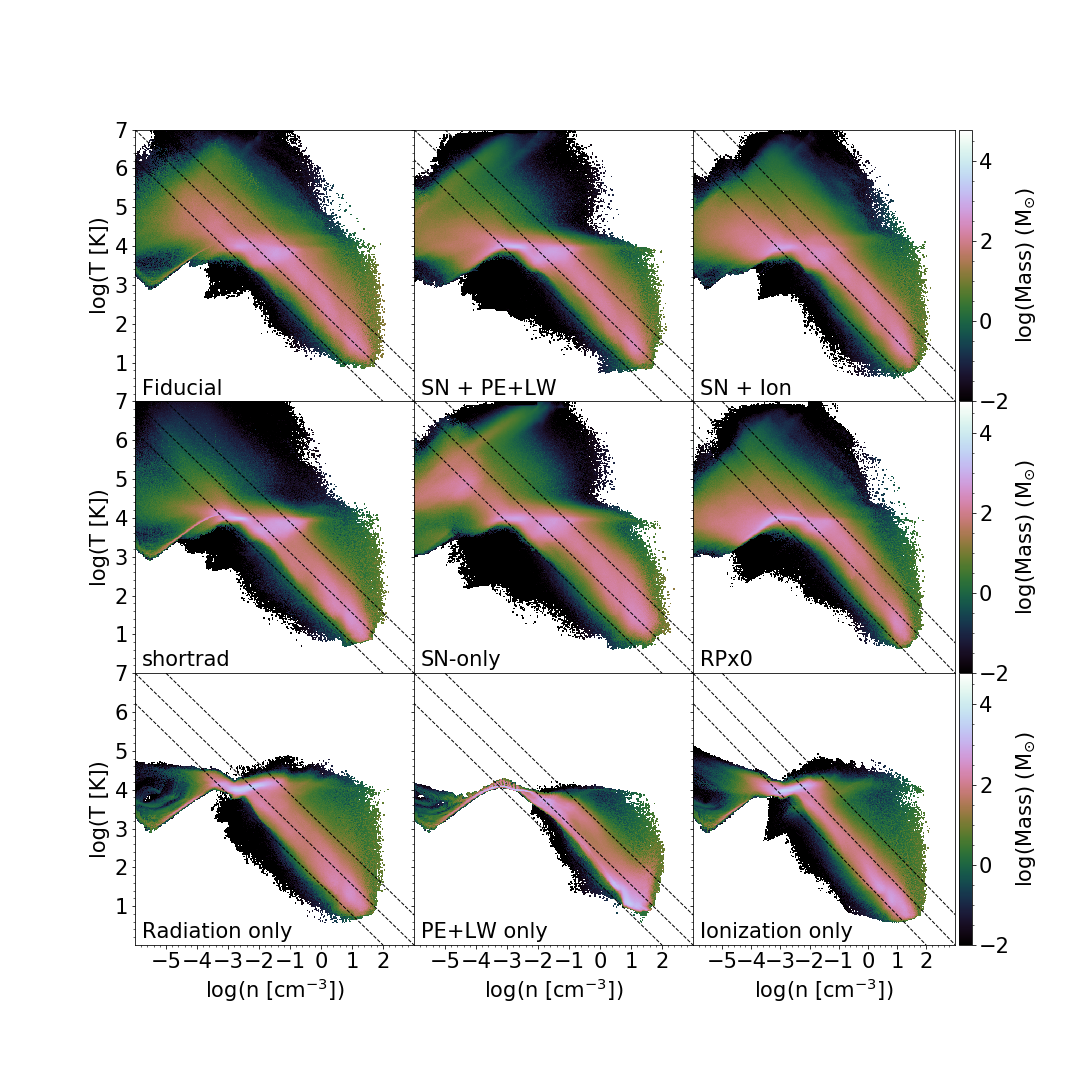
\includegraphics[width=0.95\linewidth]{figures/phase_plot_nT_phase_disk}
  \caption{The temperature - density phase diagrams for each simulation averaged over the 20~Myr period from 100-120~Myr in each simulation. Lines of constant pressure are given as dashed lines.}
  \label{fig:phase_diagram}
\end{figure*}

\begin{figure*}
  \centering
  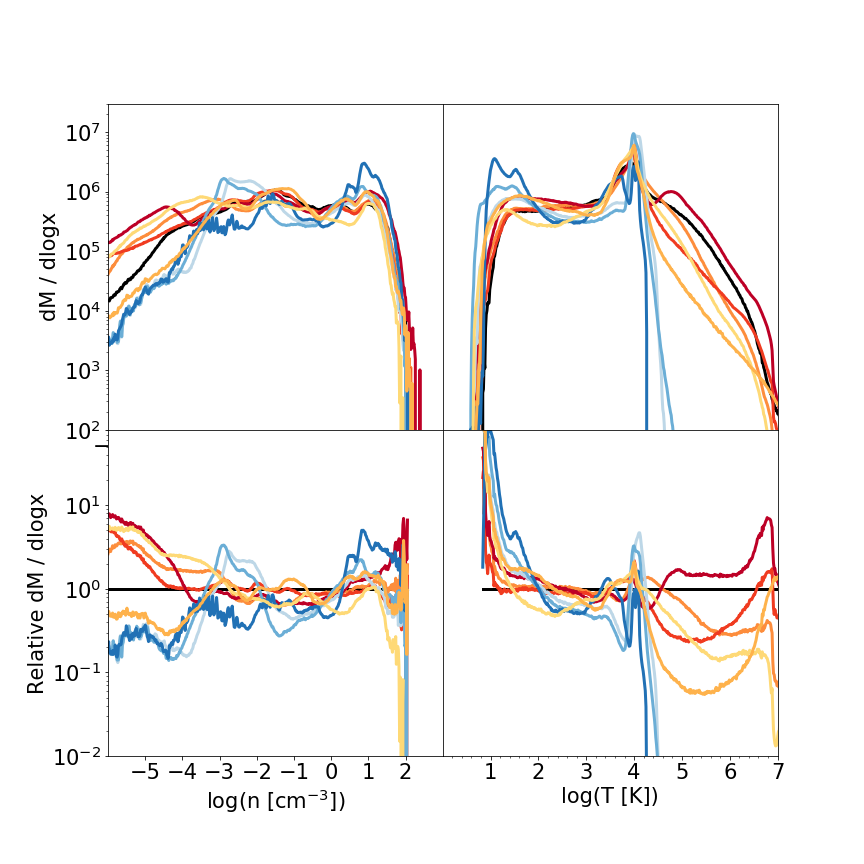
\includegraphics[width=0.95\linewidth]{figures/1D_phase_plot_2panel_nT_phase_disk}
  \caption{The 1D density and temperature PDFs (top) corresponding to Figure~\ref{fig:phase_diagram}, along with each PDF relative to the fiducial simulation (bottom).}
  \label{fig:1D_phase}
\end{figure*}


\subsection{Outflows}
\label{sec:outflows}

Galactic outflows are a natural consequence of stellar feedback, and have been demonstrated to be significant in low mass dwarf galaxies. In Figure~\ref{fig:outflow_evolution} we present the mass outflow rate as measured through an annulus with thickness 0.05~R$_{\rm vir}$ centered at two radii from the galaxy, 0.1~R$_{\rm vir}$ and R$_{\rm vir}$ (again, R$_{\rm vir}$ = 27.2kpc). The total outflow rates in the inner halo are within factors of a few during the first $\sim$200~Myr for all of the simulations except PE+LW-only, which is unable to drive significant outflows. Clearly, some combination of stellar ionizing radiation and/or supernovae are necessary to drive outflows in low mass dwarf galaxies. After this point, the runs differentiate, which periods of little-to-no outflows for the runs without any SNe, and the run with SNe, but no ionizing radiation. Interestingly, SN+Ion exhibits a larger spike in outflow rate than all other simulations after 200~Myr, likely driven by the increased SFR in this run. At the virial radius, only runs with SNe are capable of driving any significant gas outflows. 

The efficiency with which stellar feedback drives outflows is often characterized using the mass loading factor, $\eta_M$, metal mass loading factor, $\eta_Z$, and energy loading factor $\eta_E$. We define each of these quantities following \cite{LiBryan2020}: $\eta_M \equiv \dot{M}_{\rm out} / \dot{M}_{\rm *}$, $\eta_Z \equiv \dot{M}_{Z,\rm{out},\rm{SN}} / \dot{M}_{Z,\rm{SN}}$, and $\eta_E \equiv \dot{E}_{\rm out}$. By definition, $\eta_Z$ is always $<$~1 and represents the fraction of SNe-synthesiszed metals that go into outflows. There is some variety in how exactly $\eta_M$ is computed in simulations, even with this definition. $\dot{M}_{\rm out}$ is the instantaneous mass outflow rate, but $\dot{M}_{\rm *}$ is rarely take to be the instantaneous star formation rate, often time-averaged on anywhere from 1 to 100~Myr. Particularly for galaxies with bursty star formation, as is the case here, exactly how $\dot{M}_{\rm *}$ is averaged can lead to a large variability in $\eta_M$. To smooth over these fluctuations, we use 100~Myr time-averaged $\dot{M}_{\rm *}$ and compute $\eta_M$, $\eta_Z$, and $\eta_E$ every 5~Myr in each simulation for both the hot ($T \geq 3 \times 10^5$~K) and cool ($T < 3\times10^5$~K) phases. We present the average of each of these quantities for each simulation over their entire run-time in Figure~\ref{fig:loading_factors}, as a function of their average star formation rate density.

In general, our simulations show significant amounts of mass and energy driven out via cooler outflows, as the hot loading factors are comparable to or much less than the cooler loading factors. This is qualitatively different from the suite of simulations presented in \cite{LiBryan2020}, where hot loading dominates. However, although there is some overlap in $\Sigma_{\rm SFR}$ between our galaxies and a few of the simulations considered in that work, our galaxy has much lower total mass. Since the virial temperature of our halo is $1.4 \times 10^4$~K, it is not surprising that both mass and energy can flow out of our galaxy without reaching temperatures above 10$^5$-10$^6$~K. Comparing each run, only the runs with supernova contain any hot outflows. In general, there is a decreasing trend with $\eta_M$ and star formation rate. However, this trend generally follows the line of constant $\dot{M}_{\rm out}$ for each simulation, suggesting that each galaxy sustains a similar total mass outflow rates, but it is just the efficiency of stellar feedback in driving those outflows that changes by including / excluding different modes of feedback. PE+LW-only is the least efficient, followed by SN-only, with runs including PE and LW radiation and SNe somewhat more efficient, and runs with ionization and SNe the most efficient. Interestingly, the radiation-only run achieves similar $\eta_M$ as our fiducial simulation and other runs with both ionization and SNe, but with smaller $\eta_Z$ and $\eta_E$. \aje{How do we differentiate between changes in outflow efficiency and just that outflows are saturated here, or, that they are so easy to generate that it is done with minimal SF+feedback, so extra SF and feedback doesn't do much?}

The total $\eta_Z$, which again represents the fraction of SNe-produced metals that outflow relative to the total produced, is fairly uniform for all runs with SNe ($\eta_Z \sim 0.5$), but significantly lower for those without ($\eta_Z \lesssim 0.1$) and zero for the PE+LW-only run. Comparing to the differences across simulations in $\eta_M$, this raises two important points: 1) while ionizing radiation alone can drive outflows in this low-mass dwarf galaxy, SNe are necessary to drive metal-enriched outflows, 2) the metal content of SNe-driven outflows in this low-mass dwarf galaxy is less sensitive to additional feedback processes than the total outflows. Cool outflows carry a majority of the metals out of the ISM of our galaxy in each simulation (as is the case for $\eta_M$), except for the SN-only which has more metals in hot outflows, typical of more massive galaxies. 

$\eta_E$ shows similar trends except that the differences in energy content between hot and cool outflows are much smaller for some of the runs, and for others $\eta_{E,h}$ exceeds $\eta_{E,c}$ by factors of a few up to almost an order of magnitude for the SN-only run. As is thee case for $\eta_M$, this ratio correlates strongly with increasing $\Sigma_{\rm SFR}$.

Finally, \citet{LiBryan2020} find a strong correlation between the $\eta_{E,h}$ and $\eta_{Z,h}$ across their examined simulations. We plot the relationship between $\eta_{E}$ and $\eta_{Z}$ and $\eta_{E,h}$ and $\eta_{Z,h}$ in Figure~\ref{fig:loading_relation} (black points) as compared to the simulations presented in \citet{LiBryan2020} (grey points). We find that there is no clear relationship with the total energy loading factors and metal loading factors of our simulations (left panel) except that including SNe feedback and ionization generally increases both quantities. Although our simulations without SNe do not contain any hot outflows, the right panel shows that our simulations exhibit a similar linear relationship between $\eta_{E,h}$ and $\eta_{Z,h}$, but at a slightly higher value ($\sim$1) than in \citet{LiByran2020} ($\sim$0.4).


\begin{figure*}
  \centering
  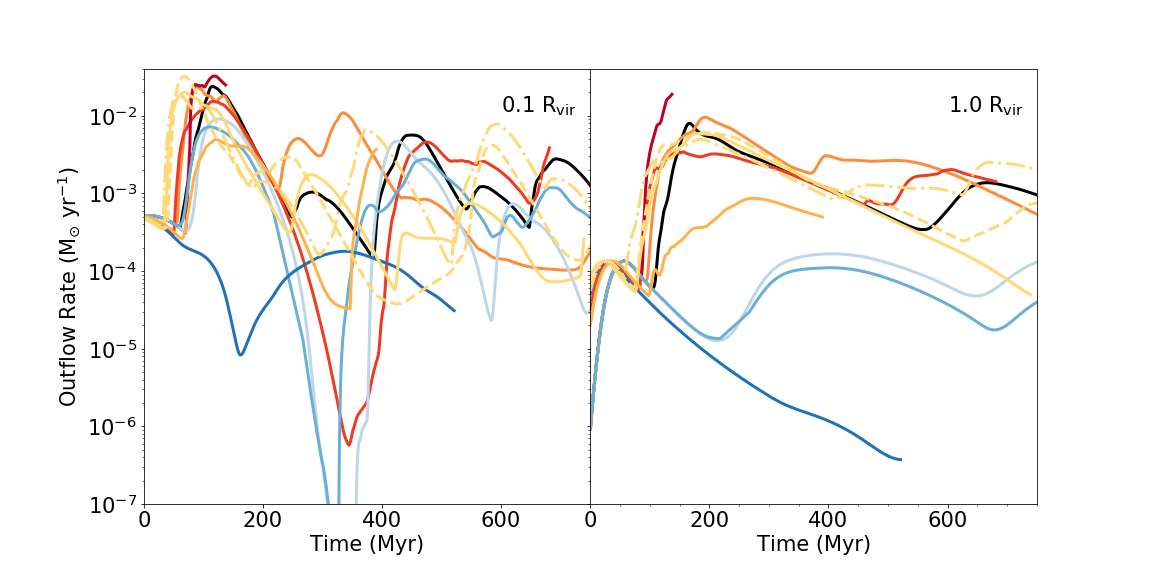
\includegraphics[width=0.95\linewidth]{figures/physics_comparison_outflow}
  \caption{The total mass outflow rate measured at different radii for each of our galaxies.}
  \label{fig:outflow_evolution}
\end{figure*}



%\begin{figure*}
%  \centering
%  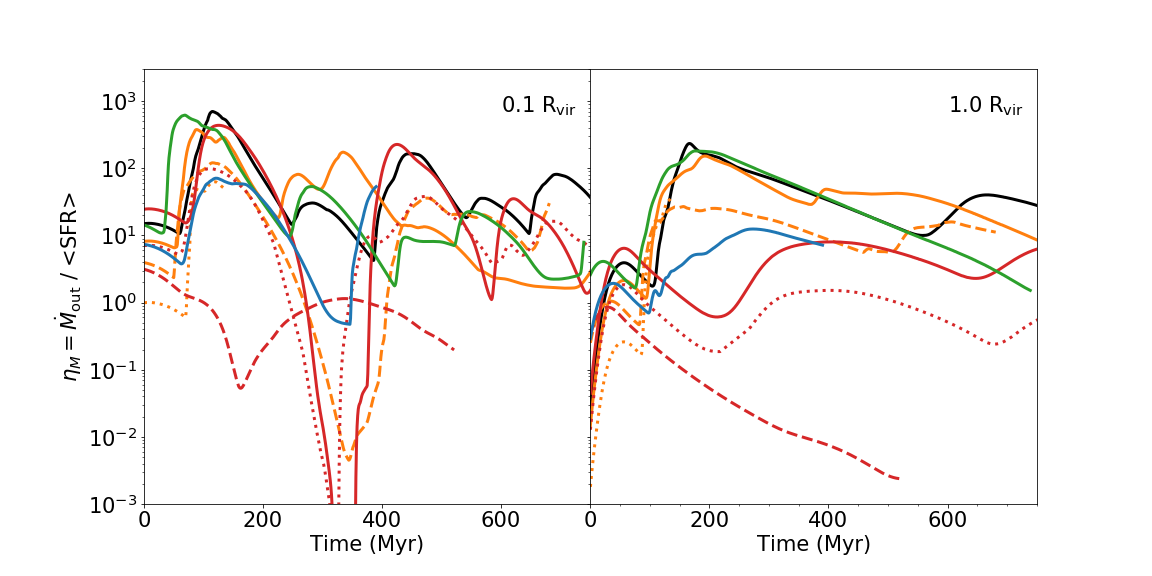
\includegraphics[width=0.95\linewidth]{figures/physics_comparison_outflow_loading}
%  \caption{The mass loading factor measured at different radii for each of our galaxies. For ease of comparison, we use the average SFR over the each entire simulation as the denominator when computing $\eta_M$.}
%  \label{fig:outflow_evolution}
%\end{figure*}

\begin{figure*}
  \centering
  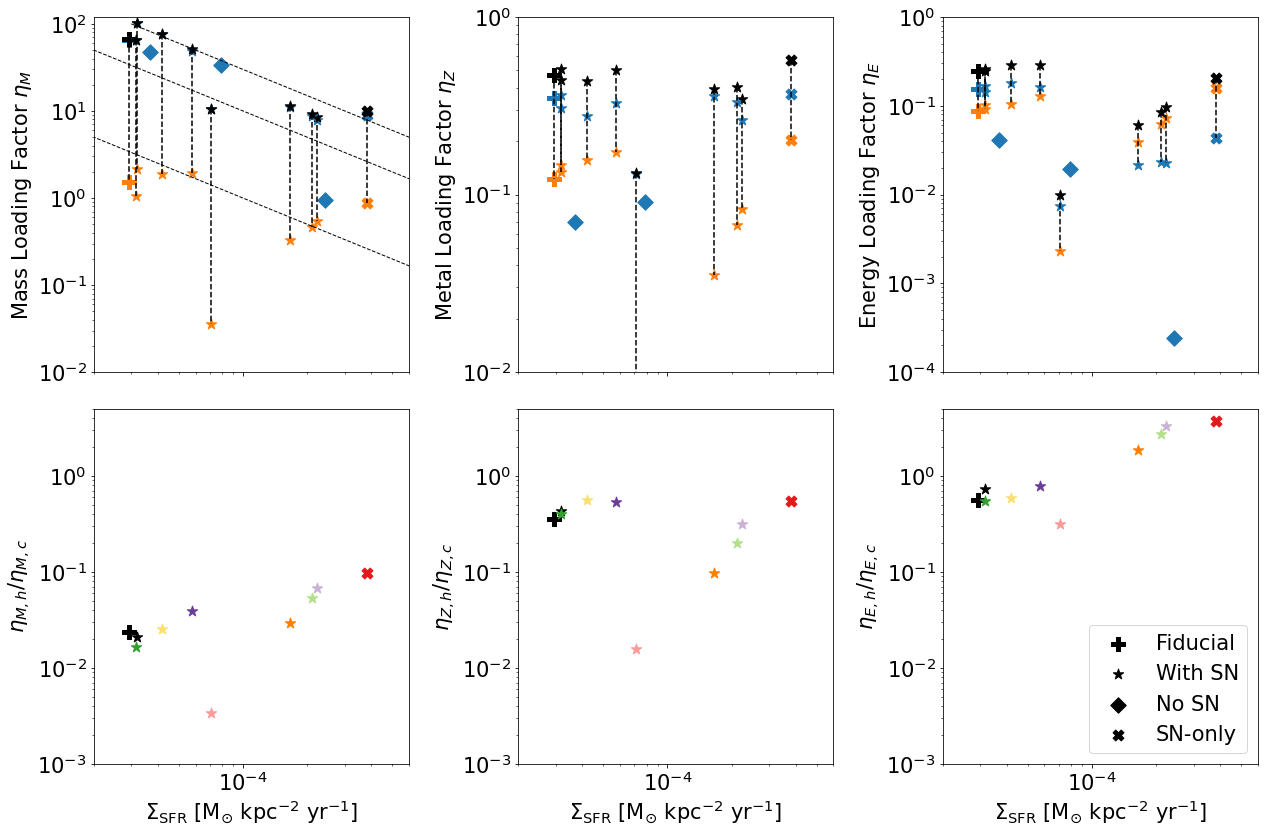
\includegraphics[width=0.95\linewidth]{figures/phys_comparison_mass_metal_hot_cold_SFR}
  \caption{The mass loading factor ($\eta_M$), metal loading factor ($\eta_Z$), and energy loading factor ($\eta_E$) for both hot (orange, $T \geq 3 \times 10^5$~K) and cold (blue, $T < 3 \times 10^5$~K) gas and their ratios for each of our simulations. The totals are shown in the top panel in black, except for the runs without SNe which contain no hot outflows and are left as blue. Each simulation is labelled, but for clarity our fiducial simulation is shown with a plus, simulations with SNe feedback as stars, those without SNe with diamonds, and SN-only with an X. For clarity, the runs without SNe are not separately labelled, but are -- in order of increasing $\Sigma_{\rm SFR}$ -- radiation-only, ionization-only, and PE+LW-only. \aje{I will add in labels by-hand to the SNe runs in final plot, but for now in order of increasing SFR the * runs are: RPx0, SN+Ion, Shortrad, SN+PE+LW} }
  \label{fig:loading_factors}
\end{figure*}

\begin{figure*}
  \centering
  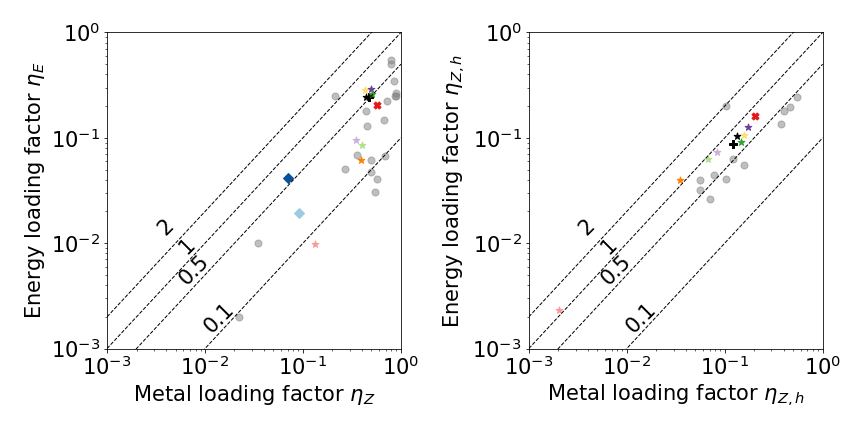
\includegraphics[width=0.95\linewidth]{figures/phys_comparison_E_loading_Z_loading}
  \caption{A comparison of the total and hot energy and metal loading factor relationships for our simulations (black points) as compared to the suite of simulations presented in \citet{LiBryan2020} (grey points), which includes data from \citet{Li2017,KimOstriker2018,Fielding2018,Hu2018,Armillotta2019,Martizzi2016} and \citet{Creasey2015}. Lines of constant $\eta_E / \eta_Z$ are shown.}
  \label{fig:loading_relation}
\end{figure*}

\subsection{Evolution of Individual Metals}
\textit{Decide if this comes before or after outflow section}

As explored in \citep{Emerick2018b}, metals released into the ISM in core collapse supernova are ejected from the galaxy through outflows at a higher efficiency than metals from AGB winds. In addition, these same metals showed smaller gas-phase abundance variations -- pointing to more efficient mixing -- than elements from AGB winds. We explore how feedback affects these differences here.

\begin{figure*}
  \centering
  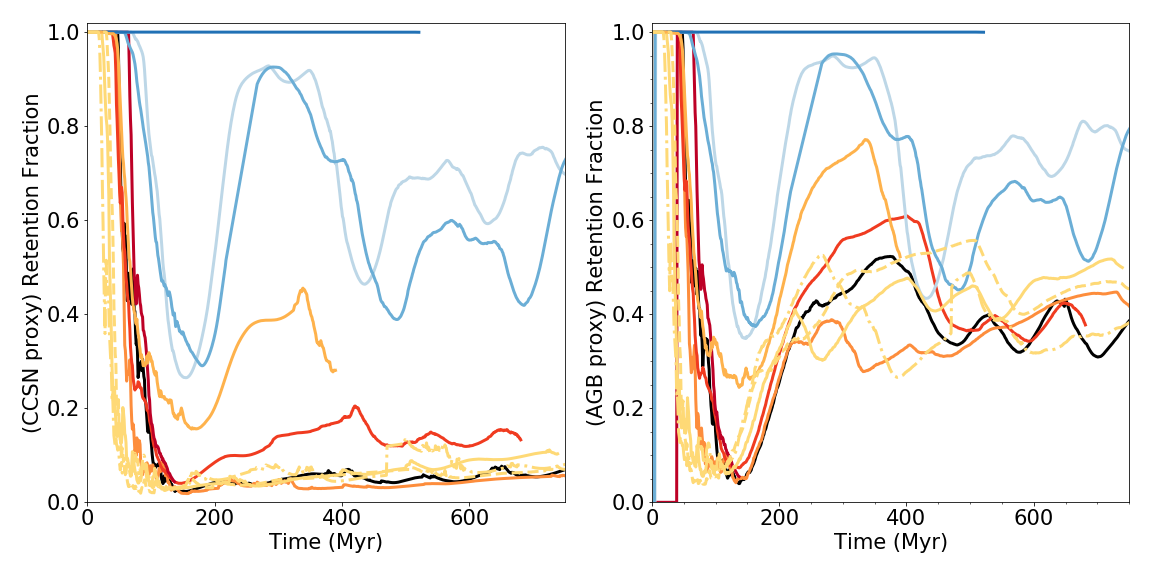
\includegraphics[width=0.95\linewidth]{figures/physics_comparison_retention}
  \caption{The retention fraction of CCSN elements (left, traced by O) and AGB elements (right, traced by Ba) in the disk of each galaxy as a function of time.}
  \label{fig:retention}
\end{figure*}

In Figure~\ref{fig:retention} we plot the fraction of metals produced that remain within the disk for a CCSN proxy (Oxygen, left) and an AGB enrichment proxy (Ba, right). The fiducial simulation shows a fairly consistent CCSN retention fraction of $\sim$5\% after the first 100~Myr. The AGB retention fraction drops during the first 100~Myr until the first AGB begin producing significant Ba; the retention fraction then grows and oscillates with the SFR, but remains around 40\%, significantly higher than that for CCSN elements. In general, runs with SN feedback show low CCSN element retention, yet that without ionizing radiation (SN+PE+LW) shows a larger retention fraction ($\sim$20\%). A similar picture is true for the AGB elements, where the SN-included runs show the lowest retention fractions. However, in all cases the AGB element retention fraction is higher than the SN element retention fraction. The runs without SN show nearly identical retention fractions for both elements. Interestingly, the two radiation runs with ionizing radiation show dramatic fluctuations in the retention fractions. These fluctuations are caused by gas that is removed beyond our formal definition of the disk region, but is not ejected far into the halo and eventually re-accretes onto the galaxy. This is additional confirmation that this difference is due in large part to the difference in energetics between the SN and AGB events, as expected from the analysis in \cite{Emerick2020a}. 

\aje{I thought this would be a cool find if the CGM / halo retention fraction (fraction of metals that stay in halo vs. leave halo entirely) was different between the two elements across runs, but it does not appear to be the case. Not showing figure here, but just discussing this point: } Although the mass of this galaxy is likely too low to observe the metal content of its circumgalactic medium, where the metals end up beyond the disk of the galaxy may also be an important discriminator between feedback models. We explore this here but for brevity the associated figure is not shown. We find that the fraction of metals in the CGM for CCSN is initially large after the first burst of star formation ($\sim$80-90\%) for all SN runs, but gradually declines to $\sim$20-30\% by the end of the simulation. Since this lost mass is not being re-accreted into the ISM, it is ejected from the halo. Although AGB elements show significantly different disk retention fractions, the CGM fractions are very similar to the CCSN elements. This is likely because whatever AGB elements do end up in the halo were carried out through the same processes as the CCSN elements, leading to the very similar evolution in the CGM.

%In Figure~\ref{fig:CGM} we plot the gravitationally bound 

\begin{figure*}
  \centering
  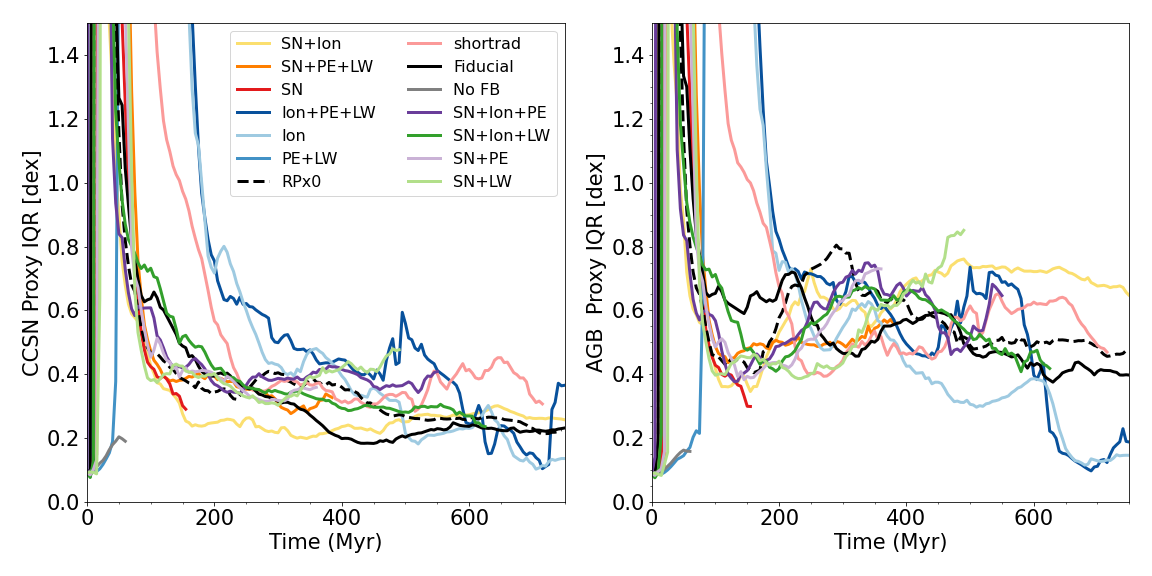
\includegraphics[width=0.95\linewidth]{figures/physics_comparison_IQR}
  \caption{A comparison of the evolution of the inner quartile range (IQR) of the gas-phase abundances of CCSN elements (left, traced by O) and AGB wind elements (right, traced by Ba) in the cold ISM (\aje{give n,T bounds}). Run Pe+LW (\pelwstyle) remains well above the vertical bounds for the duration of the simulation, and is omitted for clarity (see text).}
  \label{fig:mixing}
\end{figure*}

Finally, we explore the metal mixing differences between these runs and these two elements in Figure~\ref{fig:mixing}. We compare the inner quartile range (IQR) abundance spread of the cold gas for O, the CCSN element proxy, and Ba, the AGB element proxy, for each run. In the fiducial simulation, the CCSN elements show a declining spread throughout the evolution, reaching an IQR of $\sim$0.25 dex by the end of the simulation time. As was seen in the retention fraction, the AGB elements follow the same evolution until first produced by AGB, at which point the width rises significantly, to around 0.7~dex, and remaining well above the CCSN elements until the end of the simulation. All of the simulations including SN feedback show very similar general trends and final IQR values; the notable exception to this is the significantly larger rise in IQR in the AGB elements for run SN+Ion (\aje{not sure why... need to think...}). The comparison to the radiation only runs shows the importance that hot-phase mixing has on the evolution of these elements. While the runs with SN hit a roughly consistent IQR after the first $\sim$150~Myr, the runs without SNe take a little more than twice as long to reach this point. This is in spite of the fact that the radiation-only runs have a higher global SFR with more continual and uniformly distributed (\aje{check this}) enrichment that should allow for more rapid homogenization. However, the radiation only runs do not have SN depositing their elements first in a volume-filling hot phase, which is necessary for rapid mixing over the whole galaxy. However, ionizing radiation generates sufficiently warm / hot gas to increasing the mixing timescales of these elements. Not shown in either panel for clarity is run PE+LW, which exhibits mixing timescales on order of the dynamical time of this galaxy ($\sim$1~Gyr). This run has a gradually declining IQR like the rest of the simulations, but still has an exceedingly large IQR of 5~dex in both elements by the end of the simulation.

Since SN and AGB winds have the same injection energy in the radiation only runs, they exhibit very similar abundance spreads. This suggests that, not only is the mean abundance of individual elements an important discriminator between feedback models, but also the scatter in individual abundances can contain information about the stellar feedback that drives metal mixing in the ISM.


\subsection{Stellar abundances}
\label{sec:stellar abundances}

The previous discussion focused on the time evolution of the instantaneous gas-phase abundances of the simulated galaxies. But the best observable of galactic chemical evolution in low mass dwarf galaxies is their stellar abundances, which are the convolution of the instantaneous gas-phase abundance distributions and the SFR. To examine the effect of feedback on stellar abundances patterns, we plot the normalized 1D metallicity distribution functions (MDFs) for the abundance ratios [Mg/H]\footnote{The notation [A/B] represents the abundance of element A relative to B, normalized to the solar ratio, in logscale: [A/B]~$\equiv$~log$_{10}$(N$_{\rm A}$/N$_{\rm B}$)~-~log$_{10}$(N$_{\rm A,\odot}$/N$_{\rm B,\odot}$).}, [Fe/H], and [Ba/H] in Figure~\ref{fig:MDF1}.\footnote{ While our simulated galaxy is modelled after the $z=0$ properties of the Leo~P dwarf galaxy, we emphasize that these stellar abundances are likely not representative of the actual abundance patterns in a Leo P like dwarf galaxy ($M_* \sim 10^6 M_{\odot}$) given that we only capture 1~Gyr of evolution. However, this provides insight into possible abundance variations in lower mass dwarf galaxies who form a majority of their stars over timescales of $\sim$1~Gyr in the early Universe.} These columns represent typical enrichment from ccSNe, Type Ia SNe, and s-process enrichment from AGB winds respectively. However, we note that Fe only has a minor contribution from Type Ia SNe in our simulations due to their short run-times; this mostly also traces ccSNe enrichment. 

There are three general properties to compare across these MDFs: the location of the peak abundance, the width of the distributions, and the tails towards both higher and lower abundances. Comparing the runs in the top row to the fiducial simulation, each exhibits a higher peak abundance and slightly narrower distribution. Although each of these runs ejects a similar fraction of their metals out of the disk of the galaxy, the increase in abundance is due to the increase in star formation across these runs. This is interesting for the SN-only run in part because it is has the most metal rich stellar MDF, even though it has a similar total ISM metallicity (Figure~\ref{fig:properties}) as SN+PE+LW at he time in which these runs are compared, and even though SN+PE+LW has a higher retention fraction than the SN-only run (Figure~\ref{fig:retention}). This suggests that stellar feedback regulates stellar abundances in three ways. The two obvious: 1) by modifying the number of stars that form and thus the number of metals produced and 2) by driving out some fraction of those metals from the ISM, but also  -- more subtle -- 3) by determining how quickly ISM metals can be incorporated into new stars before being ejected. 

The radiation pressure varying runs show very similar MDFs as the fiducial simulation, but the shortrad run again shows an elevated peak abundance. The runs with only radiation show the highest enrichment across each abundance ratio, as they contain both the highest amount of star formation and greatest metal retention of all of the simulations. 


\begin{figure*}
  \centering
  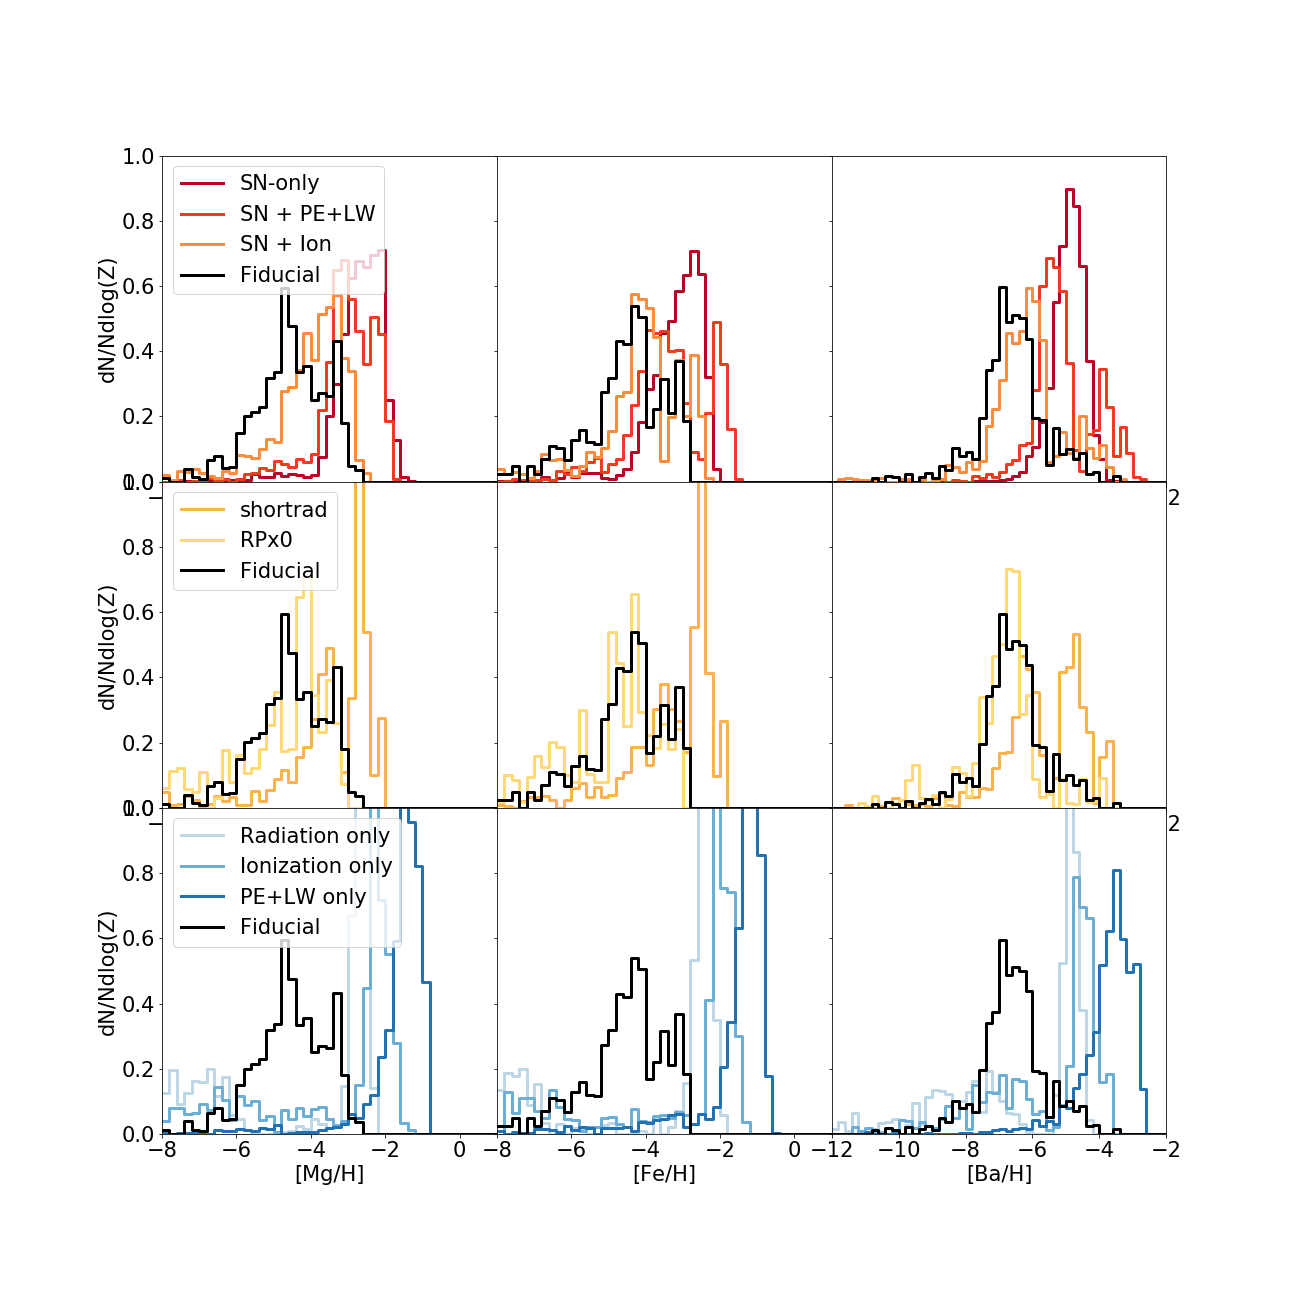
\includegraphics[width=0.95\linewidth]{figures/MgH_FeH_BaH__stellar_MDFs}
  \caption{Stellar MDFs for all stars in each simulation at t = 500~Myr (for simulations with final run times less than 500~Myr, we only take those stars that w}
  \label{fig:MDF1}
\end{figure*}

\begin{figure*}
  \centering
  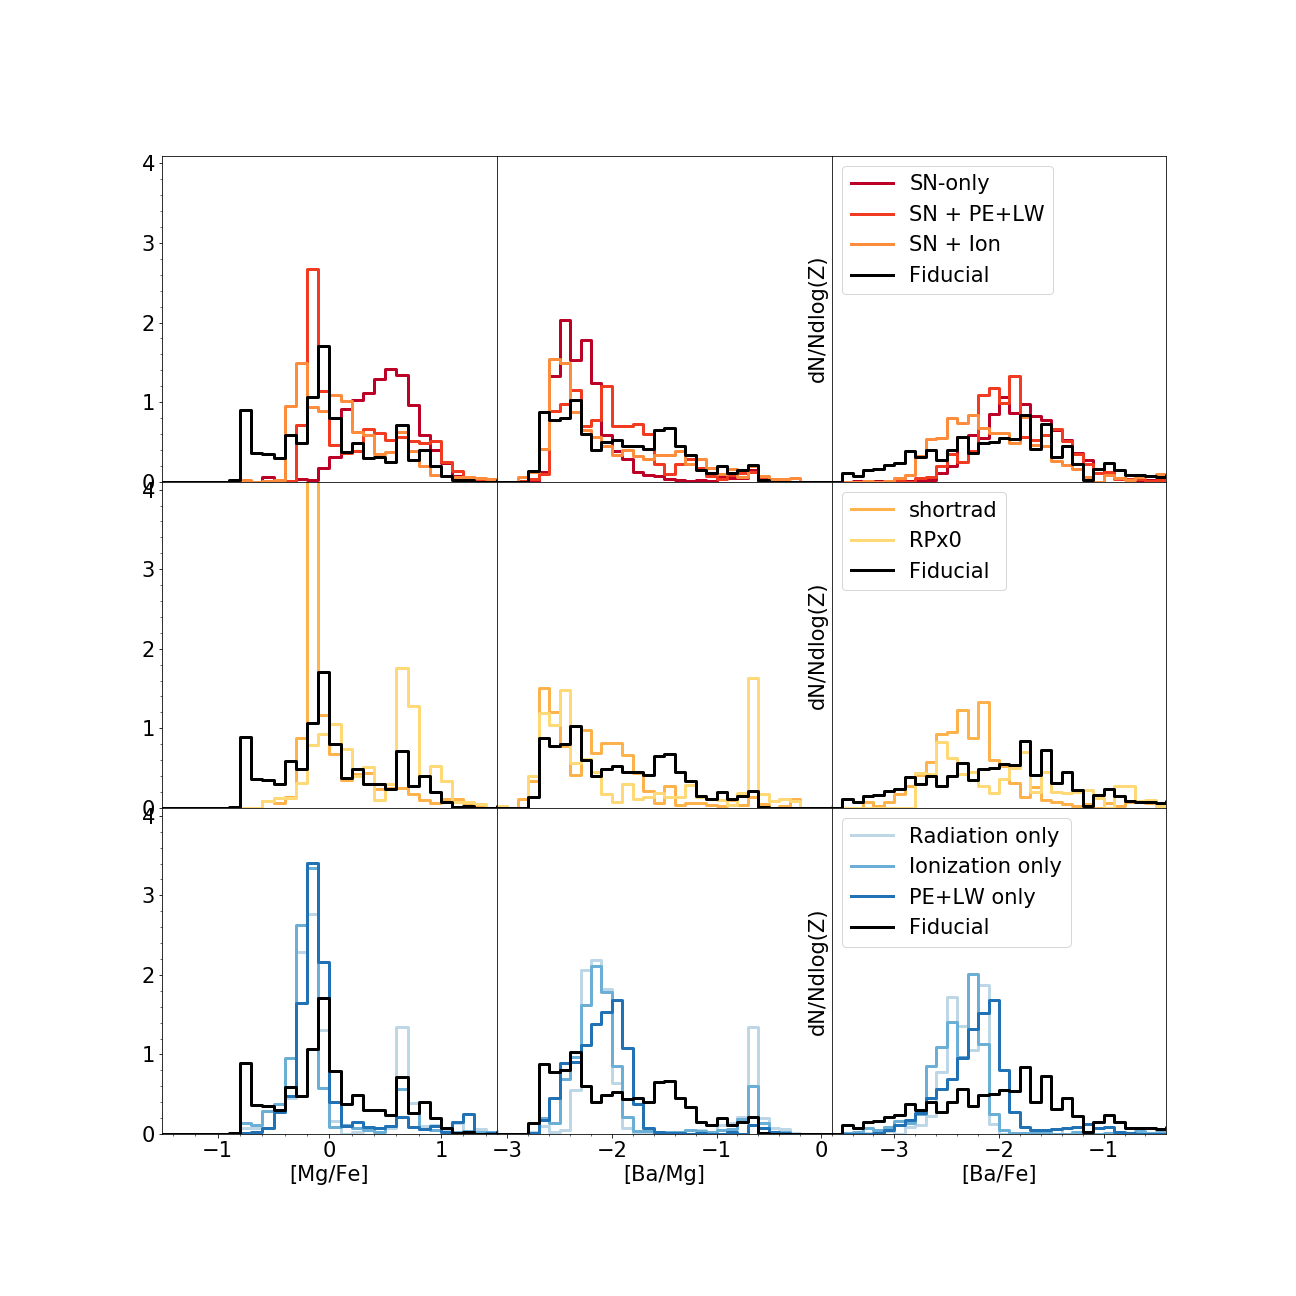
\includegraphics[width=0.95\linewidth]{figures/MgFe_BaMg_BaFe__stellar_MDFs}
  \caption{}
  \label{fig:MDF2}
\end{figure*}

\aje{For kicks, make this plot for stars formed AFTER the initial burst only....}
While the distribution of stellar abundances in terms of total metal fractions ([X/H]) provides additional insight into the effects of feedback on galactic evolution, this does not necessarily provide any additional constraints that cannot be determined by examining just the total metallicity alone. To examine if individual abundances could provide additional constraints, we plot a few abundance ratios in Figure~\ref{fig:MDF2}, [Mg/Fe], [Ba/Mg], and [Ba/Fe]. As show, there are notable differences in the widths of these distributions across runs, with the fiducial simulation generally showing the broadest variation in abundance ratios across all three abundances, but these differences are 


\subsection{Role of Photoelectric Heating}

While photoelectric heating of dust grains is an important source of heating in dense gas of more metal-rich environments like the Milky Way ISM \citep[e.g.][]{BakesTielens1994,Wolfire2003}, its role in low-metallicity dwarf galaxies is unclear. Recently, \cite{Hu2017} finds photoelectric heating to be unimportant in a galaxy with stellar mass $\sim$10$^{7}$~M$_{\odot}$ and $Z\sim$0.1~Z$_{\odot}$, in contrast to \cite{Forbes2016} who found it to be a significant source of feedback in their dwarf galaxy of similar mass and metallicity.\footnote{Though see discussion in \cite{Hu2017} which argues the difference was due to a different treatment of metal line cooling in self-shielded gas.} While our above results generally find ionizing radiation to be the more significant source of pre-SN feedback over other forms of radiation, these results always presented the effects photoelectric heating in concert with LW radiation. We examine these individually here. In Figure~\ref{fig:PELW} we compare the SFR, 

\subsection{Radiation Pressure}

\aje{Show a plot or two comparing RPx0, Fiducial, RPx2, RPx5 runs.. I'm expecting this to not be that significant}

%
% Brainstorm notes: looking at just Fiducial, no ot, no ion, no lw, no pe
%
%   OK. Taking the SN+Ion simulation (solid orange). 
%   Turning ON PE heating leads to a slightly surpressed total SF (so yes PE heating seems to have an effect on galaxy evolution, but not DRAMATIC. This has a similar Z to this run and simular total molecular H. Gas mass (HI) is also similar. So global galaxy props don't change toooo much but just surpressed SFR (just slight heating of disk)?
%
%  SN+Ion, turning ON LW (no PE) leads to FAR surpressed SF (2-3), likely due to the significantly surpressed H_2 fraction in the galaxy (early on especially but also lasting for a while). This leads to a lower ISM metallicity due partly to outflows?
%
%  Ok. here is where it gets fun. Turning BOTH on leads to a more similar evolution to just PE. Seems like LW+PE might serve to 1) kill off some H_2 which affects SF, but PE keeps disk overall stable against SF keeping SFR down as well? Turning off Ionization makes way more stars than everything.
%
% I think I'm going to have to look at a phase diagram and movie of these... really don't know.
%



\section{Discussion}

Summarize this feedback exploration in terms of both what physics is important to model but ALSO what are the general "modes" of feedback (i.e. what affects certain properties the most but also HOW each thing operates). 


\section{Conclusion}
If separate from above?

%\acknowledgments
\section*{Acknowledgments} AE was supported by ??????. \aje{CHECK IF CORRECT:} GLB acknowledges support from NSF grants AST-1615955 and OAC-1835509 and NASA grant NNX15AB20G. M-MML was partly supported by NSF grant AST18-15461. We gratefully recognize computational resources provided by NSF XSEDE through grant number TGMCA99S024, the NASA High-End Computing Program through the NASA Advanced Supercomputing Division at Ames Research Center, Columbia University, and the Flatiron Institute. This work made significant use of many open source software packages. These are products of collaborative effort by many independent developers from numerous institutions around the world. Their commitment to open science has helped make this work possible. 

%mm many citations from citebay.com.  Don't know what to cite for deepdish, so just put a placeholder in.
\software{\textsc{yt} \citep{yt}, \textsc{Enzo} \citep{Enzo2014}, \textsc{Grackle} \citep{GrackleMethod}, \textsc{Python} \citep{VanRossum1995python}, \textsc{IPython} \citep{perez2007ipython}, \textsc{NumPy} \citep{oliphant2006guide}, \textsc{SciPy} \citep{SciPy}, \textsc{Matplotlib} \citep{hunter2007matplotlib}, \textsc{HDF5} \citep{Fortner1998HDF,Koranne2011}, \textsc{h5py} \citep{h5py}, \textsc{Astropy} \citep{astropy:2013,astropy:2018}, \textsc{Cloudy} \citep{Cloudy2013}, and \textsc{deepdish}}

%\begin{figure*}
%  \centering
%  \includegraphics[width=0.45\linewidth]{figures/combined_CGM_average_evolution}
%  \includegraphics[width=0.45\linewidth]{figures/combined_CNM_average_evolution}\\
%  \includegraphics[width=0.45\linewidth]{figures/combined_CNM_average_mean-median}
%   \includegraphics[width=0.45\linewidth]{figures/combined_CNM_average_rms}
%  \caption{The same as Figure~\ref{fig:CGM_CNM} and Figure~\ref{fig:mean-median}, but comparing across both sets of runs with different SFRs. Line color corresponds to a fixed enrichment energy event, while the solid lines correspond to the higher SFR runs discussed throughout this work, and the dashed lines the lower SFR runs. See text for more details.}
%  \label{fig:SFR_comparison_CGM_CNM}
%\end{figure*}


%************* APPENDICES ************************%

%\section*{Acknowledgments}

%\clearpage
%\appendix - Liklely DO NOT use this command
%\setcounter{section}{0}%
%\renewcommand\thesection{\thechapter.\Alph{section}}
%\counterwithin{figure}{section}

%
% Place appendix here
%


\bibliographystyle{yahapj}
\bibliography{refs}

\end{document}
